\documentclass[conference]{IEEEtran}
\usepackage{fancyhdr}
\IEEEoverridecommandlockouts

\usepackage{cite}
\usepackage{amsmath,amssymb,amsfonts,amsthm}
\usepackage{algorithmic}
\usepackage{graphicx}
\usepackage{textcomp}
\usepackage{xcolor}
\usepackage{booktabs}
\usepackage{multirow}
\usepackage{makecell}
\usepackage{threeparttable}
\usepackage{tabularx}
\usepackage{bm}
\usepackage[caption=false]{subfig}

\theoremstyle{definition} % Sets style for subsequent \newtheorem commands
\newtheorem{definition}{Definition}[section] % Numbered by section (e.g., 1.1)

\def\BibTeX{{\rm B\kern-.05em{\sc i\kern-.025em b}\kern-.08em
    T\kern-.1667em\lower.7ex\hbox{E}\kern-.125emX}}
\begin{document}

\title{Spec-K: Adaptive Resource Allocation via Speculative Preview for Efficient MoE Inference}

\author{
\IEEEauthorblockN{Zhi Ma}
\IEEEauthorblockA{Beijing University of Posts and Telecommunications \\
Beijing, China \\
mz@bupt.edu.cn}
\and
\IEEEauthorblockN{Shigang Li\IEEEauthorrefmark{1}}
\IEEEauthorblockA{Beijing University of Posts and Telecommunications \\
Beijing, China \\
shigangli.cs@gmail.com
\thanks{\IEEEauthorrefmark{1}Corresponding author: Shigang Li}}
}

\maketitle
\thispagestyle{fancy}
\lhead{}
\rhead{}
\chead{}
\lfoot{\footnotesize{
SC26, November 15-20, 2026, Chicago, Illinois, USA
\newline 979-8-3195-4789-7/26/\$31.00 \copyright~2026 IEEE}}
\rfoot{}
\cfoot{}
\renewcommand{\headrulewidth}{0pt}
\renewcommand{\footrulewidth}{0pt}

\begin{abstract}
Inference serving for large language models (LLMs) often relies on static resource allocation---such as fixed Top-k routing in Mixture-of-Experts (MoE) models---despite substantial token-level heterogeneity. This mismatch causes systematic over-provisioning, magnified in long reasoning and batched speculative decoding.
We introduce Resource Allocation via Speculative Preview (RASP), a framework that leverages predictive signals from a draft model to guide token-level allocation before target-model verification, enabling fine-grained adjustment of compute budgets to match instantaneous demand.
As an instantiation, Spec-K applies RASP to MoE routing: it uses speculative preview to estimate token uncertainty and reallocates the Top-k budget dynamically via a minimalist policy, reducing expert computation, communication traffic, and activated expert count in batched verification---thereby improving throughput and even speculative acceptance.
Experiments on distributed MoE inference show that Spec-K achieves up to 1.72× end-to-end throughput improvement over a strong baseline, with negligible accuracy loss on complex reasoning and instruction-following tasks.
\end{abstract}

\begin{IEEEkeywords}
large language models, mixture-of-experts, speculative decoding, distributed inference
\end{IEEEkeywords}

\section{Introduction} \label{sec:introduction}

Mixture-of-Experts (MoE) has become a mainstream architecture~\cite{shazeer2017outrageously,fedus2022switch,lepikhin2020gshard,jiang2024mixtral,dai2024deepseekmoe,sun2024hunyuan} for frontier large language models, powering many recent open and closed models~\cite{comanici2025gemini,liu2024deepseek,yang2025qwen3,achiam2023gpt,team2025kimi,zeng2025glm,chowdhery2023palm}. By activating only a small subset of experts for each token, MoE enables scaling model capacity without proportionally increasing computation. In practice, such efficiency relies on \emph{fixed resource allocation policies}, most commonly token choice Top-$k$ routing~\cite{lepikhin2020gshard}, where each token selects the same number of experts.

Despite its simplicity and effectiveness, fixed resource allocation introduces a fundamental inefficiency. 
Autoregressive decoding exhibits substantial \emph{token-level heterogeneity}: some tokens are highly predictable, while others require significantly more modeling capacity. 
However, under fixed allocation, all tokens are assigned the same resource budget regardless of their difficulty. 
In MoE models, this manifests as \emph{over-provisioning}, where easy tokens unnecessarily consume expert computation and incur communication overhead. 
Under expert-parallel execution~\cite{lepikhin2020gshard} (where experts are distributed across devices), both FLOPs and dispatch/combine traffic scale approximately linearly with the routing budget, making this inefficiency particularly costly in distributed serving.

This mismatch becomes more pronounced in real-world workloads. 
In long reasoning tasks, token difficulty varies dramatically across the generation trajectory, amplifying the gap between required and allocated resources. 
In addition, when MoE is combined with speculative decoding (SD)~\cite{leviathan2023spec,chen2023spec}, the problem manifests in a different form. 
During batched verification, multiple candidate tokens activate different expert subsets, requiring the system to materialize their union, which weakens the memory-efficiency benefits of parallel verification. 
Both phenomena reflect the same underlying issue: \emph{fixed resource allocation fails to match token-level heterogeneity}.

A key observation is that this heterogeneity is not entirely latent. 
Speculative decoding naturally exposes \emph{predictive signals} before verification, as the draft model produces token-level distributions for candidate tokens. 
These signals, such as token entropy, provide a preview of token difficulty and are intrinsically aligned with the target model due to their shared language modeling objective. 
This suggests a general principle: \emph{resource allocation should adapt to token-level demand, guided by preview signals available prior to computation}.

\begin{figure}[t]
\centering
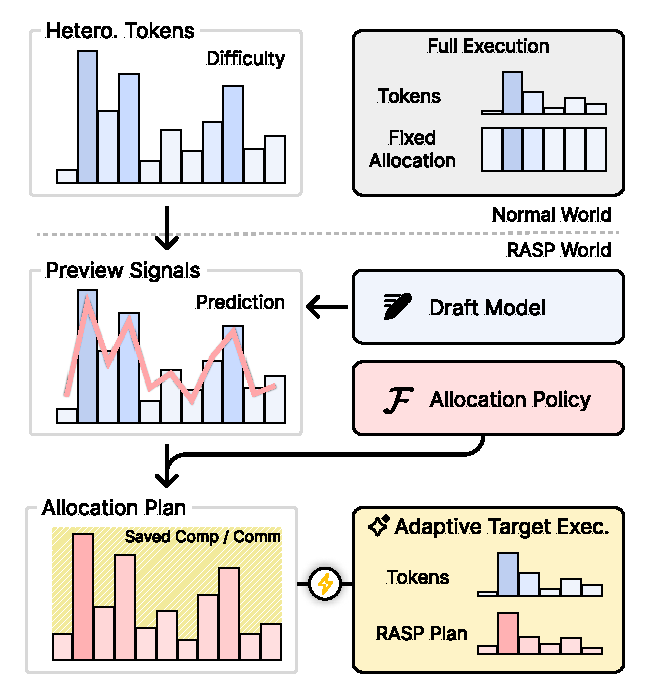
\includegraphics[width=\linewidth]{rasp_framework.pdf}
\caption{\textbf{Resource Allocation via Speculative Preview (RASP) Framework.} 
The framework consists of three components: (1) the draft model provides a \emph{preview signal} (e.g., uncertainty) for candidate tokens; 
(2) an \emph{adaptive allocation policy} maps this signal to a resource allocation plan; 
(3) the target model executes with the allocated resources, reducing waste on easy tokens. 
This abstraction decouples preview generation from policy design, enabling flexible extension to other resources (e.g., attention sparsity, layer skipping).}
\label{fig:rasp_framework}
\end{figure}

Based on this principle, we introduce \textbf{Resource Allocation via Speculative Preview (RASP)}, a general framework for adaptive inference. 
RASP decomposes the inference process into three components: (1) a \emph{preview signal} that estimates token difficulty, (2) a \emph{allocation policy} that maps this signal to a resource allocation plan, and (3) the \emph{adaptive target model execution} that realizes the allocation with speedup. 
Unlike prior adaptive mechanisms that rely on intrinsic model states (e.g., intermediate activations or router confidence), RASP is distinguished by its use of external preview signals available before target computation, enabling lightweight and training-free adaptation.
This abstraction enables fine-grained, online adjustment of compute budgets, allowing systems to allocate more resources to difficult tokens while reducing waste on easy ones. 
Beyond MoE routing, the framework naturally extends to other forms of adaptive computation, such as sparse attention or layer skipping.

As a concrete instantiation of RASP, we propose \mbox{\textbf{Spec-K}}\footnote{https://github.com/ParCIS/Spec-K.git}, a training-free dynamic Top-$k$ routing method for MoE inference.
Spec-K leverages speculative preview to estimate token uncertainty and assigns a token-wise routing budget accordingly. 
By increasing Top-$k$ for uncertain tokens and reducing it for predictable ones, Spec-K implements a simple yet effective adaptive allocation mechanism during speculative verification. 
The policy itself is minimalist---a piecewise constant function mapping perplexity to routing budget---making it both interpretable and easy to optimize.
This design preserves model quality while reducing unnecessary expert activation.

Such adaptive allocation yields multiple system-level benefits. 
Reducing the routing budget directly lowers expert-side computation (FLOPs) and dispatch/combine communication. 
At the same time, dynamically shrinking per-token expert sets reduces the union of activated experts across tokens in batched verification, improving memory locality and efficiency. 
In practice, concentrating resources on uncertain tokens can also improve speculative acceptance rates, further amplifying throughput gains.

In summary, we make the following contributions:

\begin{itemize}
    \item We propose \textbf{Resource Allocation via Speculative Preview (RASP)}, a general framework for adaptive LLM inference. RASP addresses the fundamental misalignment between fixed resource allocation and token-level heterogeneity---a mismatch amplified in long reasoning and speculative decoding workloads---by leveraging preview signals to enable token-level adaptation before target computation. (Sec.~\ref{sec:method:rasp_framework})

    \item We present \textbf{Spec-K} as a practical instantiation of RASP for MoE routing, using a simple and training-free policy to dynamically adjust Top-$k$ based on token uncertainty. (Sec.~\ref{sec:method:spec_k})

    \item We provide analysis (Sec.~\ref{sec:mechanism}) and an automatic search procedure (Sec.~\ref{sec:method:autosearch}) to identify high-quality operating points under the quality–efficiency trade-off.

    \item We demonstrate that Spec-K achieves up to $1.72\times$ end-to-end throughput improvement over a strong distributed MoE baseline, with negligible accuracy degradation on complex reasoning and instruction-following benchmarks. (Sec.~\ref{sec:evaluation})
\end{itemize}


\section{Background and Motivation}

\subsection{Mixture-of-Experts and Serving}

Mixture-of-Experts (MoE) replaces the dense feed-forward network in transformer layers with a set of $n$ experts, where only a sparse subset is activated for each token.
For a token representation $\mathbf{x}_{L,i}$ at layer $L$, the gating function produces routing scores over all experts. Under token-choice routing~\cite{lepikhin2020gshard}, let $\mathcal{S}_{L,i}$ denote the selected Top-$k$ expert set; the corresponding expert outputs are combined to form the layer output.

In distributed inference, MoE layers are typically executed under an expert-parallel paradigm. The forward pass of a single MoE layer can be decomposed into four stages:
\begin{itemize}
    \item \textbf{Routing}: compute gating scores and select Top-$k$ experts for each token.
    \item \textbf{Dispatch}: send token representations to the devices hosting the selected experts.
    \item \textbf{Expert Computation}: apply the SiLU-Mul activation from SwiGLU~\cite{shazeer2020glu} and two GEMMs, often implemented with grouped general matrix multiplication (GroupGEMM~\cite{gale2023megablocks}) to improve hardware utilization.
    \item \textbf{Combine}: the inverse operator of dispatch, gather and aggregate expert outputs back to the original token order.
\end{itemize}

Both dispatch and combine incur all-to-all communication across devices, while expert computation scales with the total number of token-expert assignments.
For a batch of tokens indexed by $i$, the system workload also depends on the set of activated experts across all tokens. Define the union:
\begin{equation*}
\mathcal{U}_L = \bigcup_i \mathcal{S}_{L,i}.
\end{equation*}
The size of $\mathcal{U}_L$ determines how many experts must be materialized during execution, directly impacting memory footprint, communication volume, and the efficiency of grouped execution.

The aggregate assignment count is not the only determinant of latency.
Since experts execute in parallel, the most heavily loaded device can determine the critical path, making the distribution of assignments across devices relevant as well.

In practice, both communication cost and expert computation scale approximately linearly with the routing budget $k$, making Top-$k$ a key control knob for system efficiency.

\subsection{Speculative Decoding}

Speculative decoding (SD) accelerates autoregressive generation by using a lightweight draft model to propose multiple candidate tokens, which are then verified in parallel by a larger target model~\cite{stern2018blockwise,leviathan2023spec,chen2023spec}.

At each decoding step, the draft model generates a sequence of $\gamma$ candidate tokens $\{S_1, \dots, S_\gamma\}$. The target model evaluates these tokens in a single forward pass, and accepts a prefix based on agreement between the draft and target distributions. The process then continues from the first rejected token.

This procedure enables multiple tokens to be processed per target forward pass, improving efficiency when the acceptance rate is high. The benefit primarily comes from amortizing model execution and memory access across candidate tokens.

During verification, the target model processes $1+\gamma$ tokens in parallel (including one carried-over token from the previous step). In MoE models, each of these tokens may activate a different subset of experts. For batched verification, let $b$ index requests and $i=1,\dots,1+\gamma$ index positions in each verification block; $\mathcal{S}_{L,b,i}$ denotes the corresponding selected expert set. The effective expert set becomes
\begin{equation*}
\mathcal{U}_L^{\text{SD}} = \bigcup_b \bigcup_{i=1}^{1+\gamma} \mathcal{S}_{L,b,i},
\end{equation*}
which can be significantly larger than that of a single token. This increases communication overhead in dispatch/combine and reduces the efficiency of grouped expert execution.

\subsection{Entropy, Perplexity, and Uncertainty}
\label{sec:bg:uncertainty}

The predictive distribution of a language model provides an intrinsic measure of uncertainty regarding the next token.
Given the model's output probability distribution $\mathbf{p}_i$ over the vocabulary $\mathcal{V}$ at step $i$, the Shannon entropy is defined as:
\begin{equation*}
H(\mathbf{p}_i) = -\sum_{w \in \mathcal{V}} p_i(w) \log p_i(w).
\end{equation*}

The corresponding token-level perplexity is derived as the exponential of the entropy:
\begin{equation*}
\text{PP}(\mathbf{p}_i) = \exp(H(\mathbf{p}_i)).
\end{equation*}

While entropy quantifies the average information content, perplexity provides a more intuitive physical interpretation: it represents the \textit{effective size} of the model's choice set. Specifically, it can be interpreted as the number of equally likely token choices that would produce the same entropy. In the context of speculative decoding, these metrics characterize the ``sharpness'' of the draft model's distribution prior to verification, where lower perplexity implies significant information redundancy, suggesting that the distribution is more robust to lossy approximations or high-ratio compression during distributed inference.

\subsection{Long Reasoning and Token Heterogeneity}

In long-form generation tasks such as chain-of-thought reasoning, token-level behavior exhibits substantial heterogeneity. 
Sequences typically contain a mix of predictable tokens (e.g., formatting or intermediate steps) and high-uncertainty tokens that determine the direction of reasoning.

Recent studies indicate that a relatively small fraction of tokens with high uncertainty plays a disproportionate role in shaping model outputs~\cite{wang2025beyond8020}. 
At the same time, long reasoning workloads are dominated by decoding, making per-token efficiency a primary factor in overall system performance.

This heterogeneity is reflected both in model behavior and in system workload, particularly in settings where multiple tokens are processed jointly, such as speculative decoding.

\begin{figure*}
    \centering
    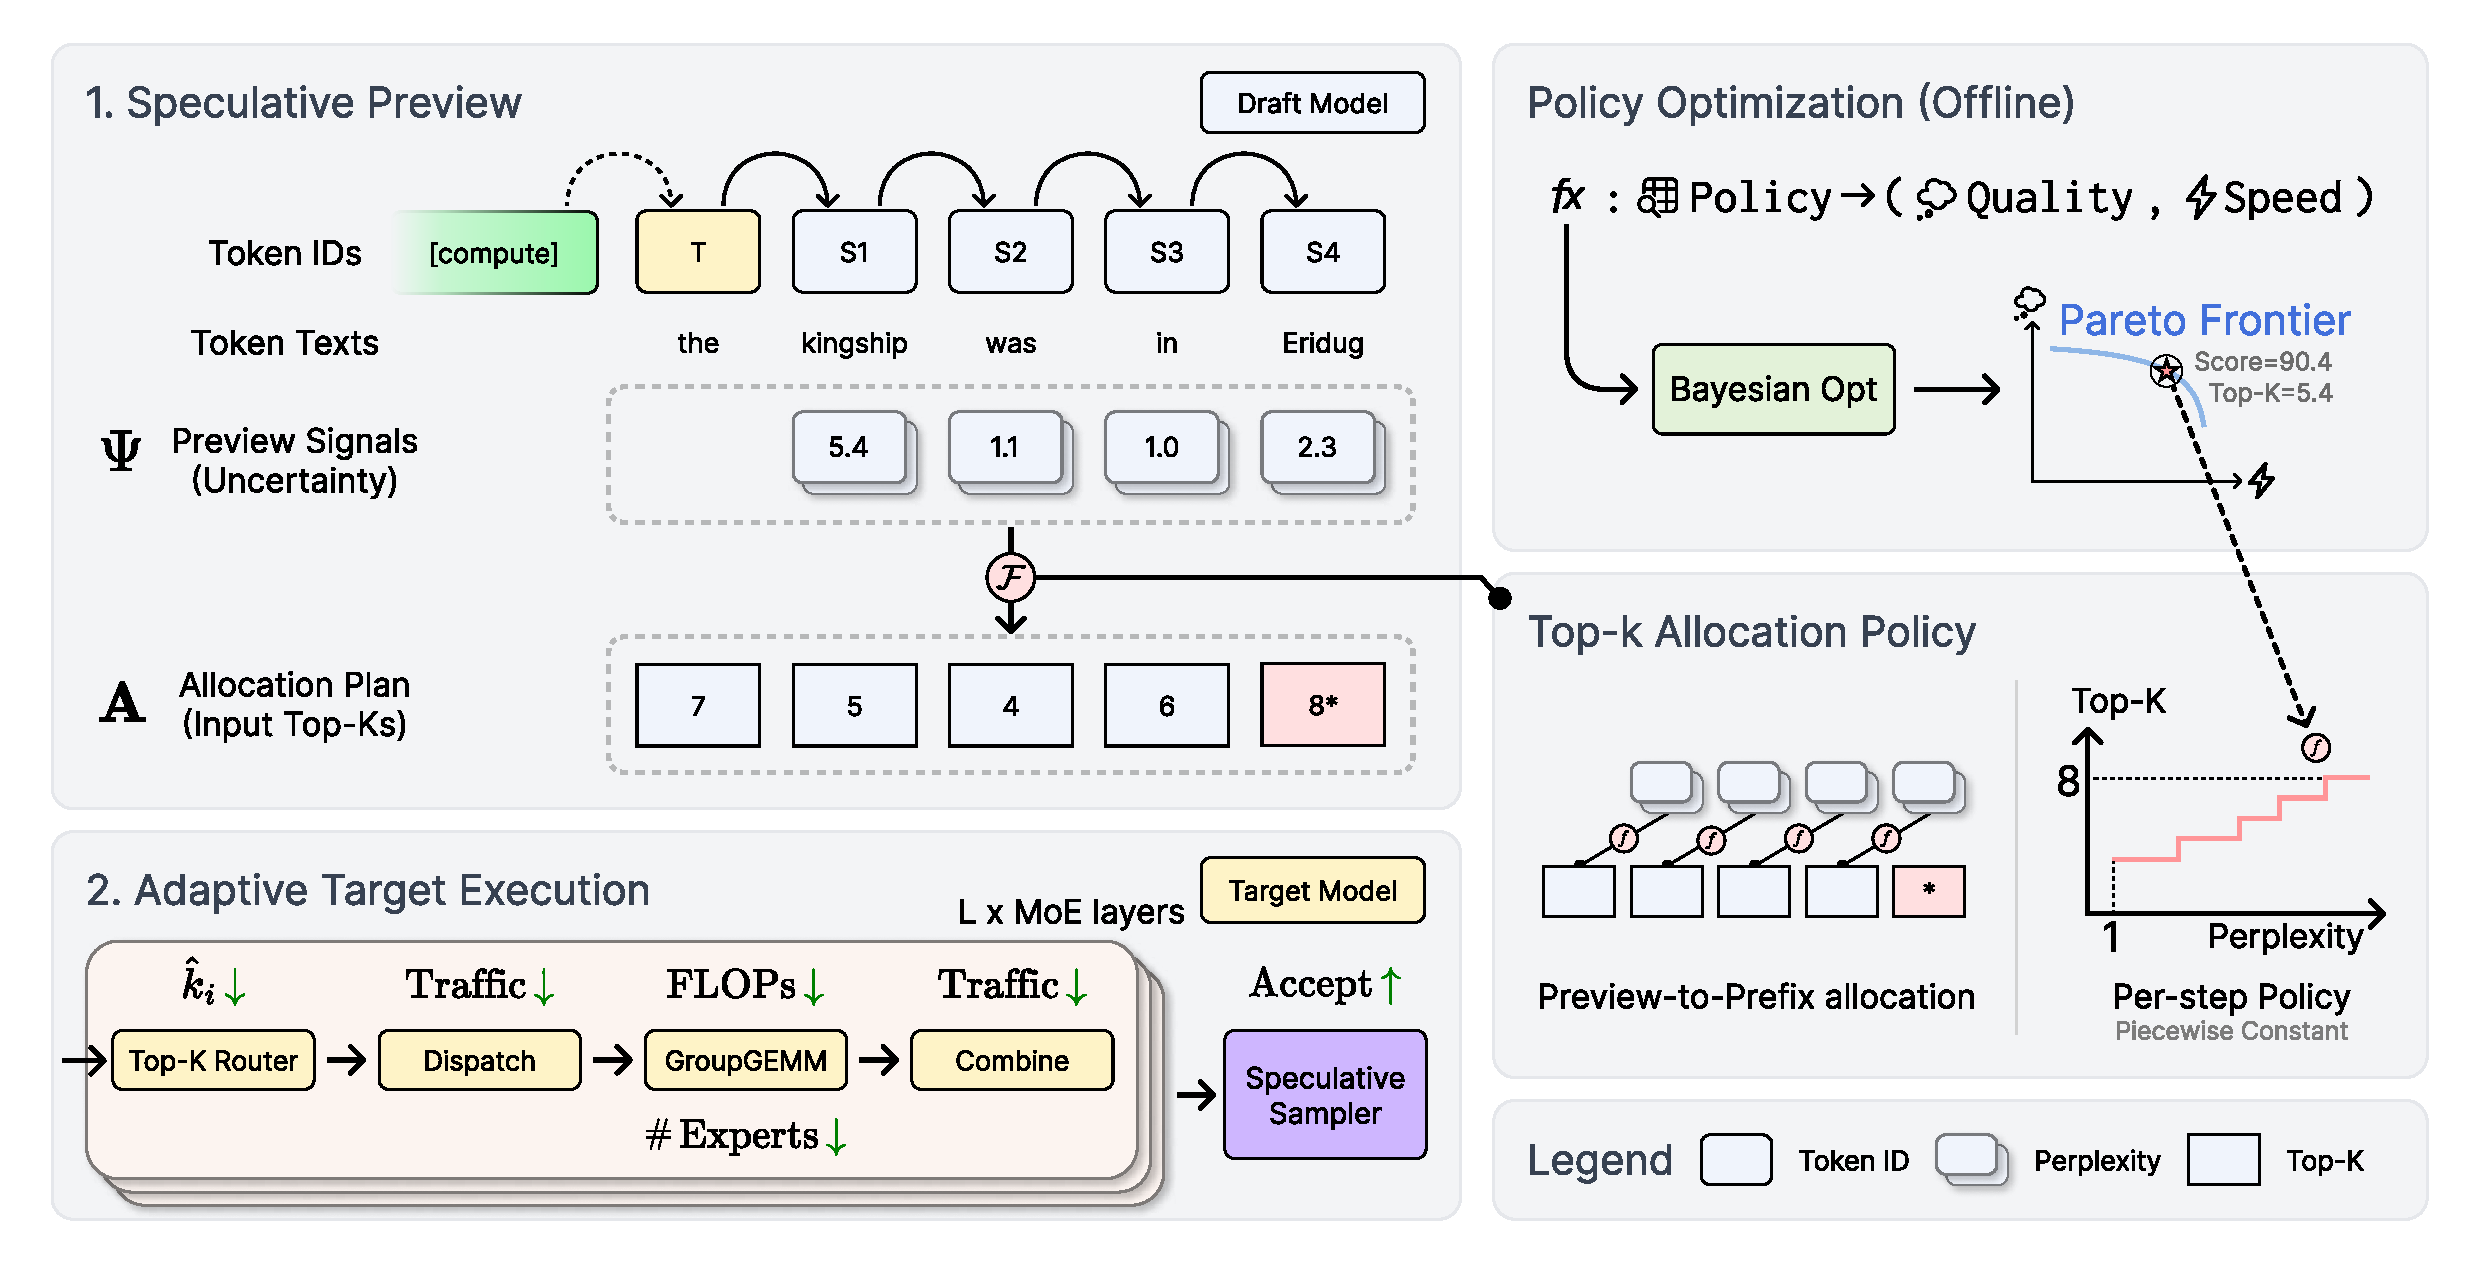
\includegraphics[width=1\linewidth]{workflow.pdf}
    \caption{Overview of \textbf{Spec-K,} an instantiation of RASP for MoE dynamic Top-$k$. 
A draft model provides preview signals that an allocation policy maps to a token-wise routing plan, enabling dynamic resource allocation during MoE verification. 
This adaptive mechanism yields systematic speedups through reduced computation and communication.}
    \label{fig:workflow}
\end{figure*}

\section{Methodology} \label{sec:methodology}

\subsection{RASP: Resource Allocation via Speculative Preview} \label{sec:method:rasp_framework}

We formalize \textbf{Resource Allocation via Speculative Preview (RASP)} as a general framework for adaptive inference under token-level heterogeneity. 
In a verification step, the target model processes one prefix token and $\gamma$ draft-generated candidates $S_1,\dots,S_\gamma$; RASP uses speculative preview to allocate computation before target execution.

\begin{definition}[Preview Signal]
A \emph{preview signal} $\Psi$ is obtained from the draft model before target execution. 
$\Psi$ encodes information about token-level difficulty and may take arbitrary structure. 
Examples include per-token scalars (e.g., predictive entropy or perplexity), attention score matrices, router logits, or hidden states. 
We treat $\Psi$ as an abstract signal to emphasize that allocation operates on its semantics rather than its representation.
\end{definition}

\begin{definition}[Allocation Policy]
An \emph{allocation policy} $\mathcal{F}$ maps a preview signal $\Psi$ to an \emph{allocation plan} $\mathbf{A}$:
\begin{equation}
\mathbf{A} = \mathcal{F}(\Psi).
\end{equation}
The policy may exploit arbitrary structure in $\Psi$, including token-wise independence or cross-token interactions. 
Crucially, $\mathcal{F}$ is decoupled from model parameters, enabling independent design and optimization.
\end{definition}

The output of $\mathcal{F}$ is an \emph{allocation plan} $\mathbf{A}$, which specifies how computational resources are distributed across tokens. 
Its structure depends on the adaptation target: a vector of expert counts for MoE routing, a collection of layer subsets for early exit, or attention masks for sparse attention. 
The target model interprets $\mathbf{A}$ to modulate per-token resource usage, while model weights remain unchanged.

Executing with plan $\mathbf{A}$ incurs a system cost $\mathcal{C}(\mathbf{A})$, whose form depends on the resource being controlled. 
For a given workload distribution, adaptive allocation seeks to minimize the expected system cost $\mathbb{E}[\mathcal{C}(\mathbf{A})]$ under a quality constraint.

RASP defines a compositional design space over the preview signal $\Psi$, allocation policy $\mathcal{F}$, and allocation plan $\mathbf{A}$; its uncertainty-guided MoE instantiation is \textbf{Spec-K}.

\subsection{Spec-K: A Dynamic Top-k Instantiation} \label{sec:method:spec_k}

We instantiate RASP for MoE routing with \textbf{Spec-K}, a dynamic Top-$k$ allocation mechanism driven by speculative preview.
This instantiation makes three concrete design choices for the RASP components.
First, the \textbf{preview signal} $\Psi$ is instantiated as token-level uncertainty derived from the draft model, represented as a vector $\boldsymbol{\Psi} = (\psi_1,\dots,\psi_\gamma)$.
Second, the \textbf{resource} being controlled is the routing budget in MoE layers---the Top-$k$ number of activated experts per token.
Third, the \textbf{allocation policy} $\mathcal{F}$ produces a token-wise plan $\mathbf{A} = (\hat k_1,\dots,\hat k_{1+\gamma})$, where each $\hat k_i \in \{0,\dots,k\}$ specifies the budget for token $i$. We next elaborate on these choices.

For each candidate token $S_i$, let $\mathbf{p}_i$ denote its predictive distribution from the draft model.
We compute the preview signal as its perplexity:
\begin{equation}
\psi_i = \exp(H(\mathbf{p}_i)), \quad i = 1,\dots,\gamma.
\end{equation}
This choice of signal extracts a highly interpretable, compressed representation of token difficulty from the rich, high-dimensional information available in the draft model's forward pass (e.g., hidden states or attention patterns).
We analyze the advantages of this uncertainty-based signal in Sec.~\ref{sec:mechanism}, showing that it provides a principled basis for allocation by identifying tokens where approximation is naturally more tolerable.

The allocation policy then maps this signal vector $\boldsymbol{\Psi}$ to a resource allocation plan $\mathbf{A}$:
\begin{equation}
\mathbf{A} = \mathcal{F}(\boldsymbol{\Psi}) = (\hat k_1,\dots,\hat k_{1+\gamma}).
\end{equation}

Given the allocation plan $\mathbf{A}$, we realize dynamic routing by modifying the standard Top-$k$ gating mechanism in each MoE layer. For token $i$ at an arbitrary MoE layer, let $\mathcal{G}_{i,j}$, $j=1,\dots,k$, denote the routing weight at the $j$-th position of the standard Top-$k$ output, ordered by decreasing gate score. Spec-K applies zero-masking to this ordered output according to the allocated budget~$\hat k_i$:
\begin{equation}
\hat{\mathcal{G}}_{i,j} =
\begin{cases}
\mathcal{G}_{i,j}, & 1\le j\le\hat{k}_i,\\
0, & \hat{k}_i<j\le k.
\end{cases}
\end{equation}
Thus, a token with budget $\hat k_i$ activates only its top $\hat k_i$ experts while leaving the retained routing weights unchanged.

The benefits of this adaptive allocation are directly reflected in the system cost $\mathcal{C}(\mathbf{A})$.
In MoE routing, both expert computation (FLOPs) and dispatch/combine communication scale approximately linearly with the number of activated experts.
Consequently, the resource cost of a verification step satisfies $\mathcal{C}(\mathbf{A}) \propto \sum_{i=1}^{1+\gamma} \hat k_i$.
By reducing $\hat k_i$ for low-uncertainty tokens, Spec-K directly lowers both the computational load and the cross-device communication traffic during verification.

In practice, this preview-guided allocation can also improve speculative acceptance 
rates, further amplifying throughput gains, as we will show in our evaluation.

This instantiation defines the interface and input-output behavior of the allocation policy $\mathcal{F}$.
The detailed, structured design of this policy function is presented in the next section.

\subsection{Allocation Policy Design} \label{sec:method:policy}

The allocation policy $\mathcal{F}$ serves as the core component of Spec-K, governing the trade-off between model quality and system efficiency.
While speculative decoding exposes a rich set of signals (e.g., attention patterns or routing logits), we adopt a \emph{minimal and structured design} that directly maps token uncertainty to routing sparsity.

Specifically, we implement $\mathcal{F}$ as a \textit{preview-to-prefix allocation}: 
the uncertainty of each candidate token determines the routing budget of its preceding 
context token---the one from which it was drafted.
Let $f(\psi_i)$ denote the \textit{per-step policy} that maps a single preview signal 
to a routing budget. The overall allocation is then defined by applying $f$ 
to each candidate's preview, with a shift:
\begin{equation}
\mathcal{F}(\boldsymbol{\Psi}) := (f(\psi_1),\; f(\psi_2),\; \dots,\; f(\psi_\gamma),\; k)
\end{equation}
The final token is assigned the default budget $k$, as its preview signal is not 
available prior to verification.

We parameterize the per-token function $f(\cdot)$ as a \textit{piecewise constant function} over the uncertainty signal $\psi_i$:
\begin{equation}
f(\psi_i) :=
\begin{cases}
k, & \psi_i \ge a_k, \\
k-1, & a_{k-1} \le \psi_i < a_k, \\
\quad \vdots \\
1, & a_1 \le \psi_i < a_2, \\
0, & \psi_i < a_1,
\end{cases}
\end{equation}
where the thresholds are monotonic and satisfy:
\begin{equation}
a_1 \le a_2 \le \cdots \le a_k.
\label{eq:monotonicity}
\end{equation}

This parameterization defines a compact yet expressive policy space.
It is motivated by three considerations:
\begin{itemize}
    \item \textbf{Simplicity}: the policy is low-dimensional and easy to find a near-optimal allocation rule.
    \item \textbf{Coverage}: it spans a wide range of behaviors, from static Top-$k$ to aggressively sparse routing.
    \item \textbf{Interpretability}: the piecewise constant form yields an explicit, rule-like mapping from preview signal to allocation decision, making the behavior easy to reason about.
\end{itemize}

The monotonicity constraint enforces that higher-uncertainty tokens receive more experts, which improves stability while only mildly restricting expressiveness.

Given this parameterization, the remaining question is how to select an optimal policy under the quality–efficiency trade-off.
We address this via an automatic search procedure described next.

\subsection{Policy Optimization} \label{sec:method:autosearch}

Selecting the thresholds in $f(\cdot)$ determines how routing sparsity adapts to token uncertainty, and thus directly controls quality and efficiency.
This defines a search function that maps policy to (quality, speed), and induces a two-objective optimization problem over these two metrics.
Its solution is characterized by a Pareto frontier, which exposes a diverse set of operating points, allowing users to select a policy that matches their desired trade-off.

The search is performed over the threshold parameters $\{a_i\}$ in $f(\cdot)$, which carry the monotonicity constraint in Eq.~(\ref{eq:monotonicity}).
To optimize over this constrained space, we represent the thresholds as cumulative products, with the first factor setting the largest threshold and each subsequent factor constrained to $[0,1]$; the ordering of $\{a_i\}$ is then ensured by construction.

During offline calibration, we use a standard multi-objective Bayesian optimization procedure to explore this space, implemented with Gaussian process-based optimization in BoTorch~\cite{balandat2020botorch} and a hypervolume-based acquisition function.
Each candidate policy is evaluated using an automated benchmarking pipeline based on~\cite{gao2024evalharness}, returning both benchmark score and average Top-$k$.

In practice, we use a low-dimensional parameterization (typically 5--6 parameters for $k=8$ by disabling the leading over-aggressive positions), which keeps the search efficient; the overall cost is dominated by model inference during evaluation.

We note that for architectures with built-in redundancy, such as models with shared 
experts, allocation policies with aggressively low Top-$k$ may be achievable without 
quality degradation. An instance of this (DeepSeek-R1 with MTP) is shown in our evaluation
(Sec.~\ref{sec:evaluation:pareto}).

\subsection{Operating Principles of Spec-K}
\label{sec:mechanism}

Beyond its routing rule, Spec-K exhibits a special system-level behavior: it applies approximation when decoding is naturally tolerant, and becomes more conservative as uncertainty increases.
This subsection develops a mechanistic account of that behavior.

A full end-to-end perturbation analysis of modern transformers would be intractable and offer limited insight, given the highly nonlinear interaction among attention, MLP, and residual connections.
We therefore focus on two tractable views of the same behavior: a per-step view based on \emph{local sensitivity} in autoregressive decoding, and a sequence-level view based on \emph{self-regulation} under uncertainty-aware routing.

\subsubsection{Local Sensitivity of Autoregressive Decoding}

Spec-K is most aggressive when the current decoding step is predicted to be easy, namely when the speculative candidate has low perplexity.
This choice can be understood through a basic robustness property of autoregressive decoding.

Consider decoding step $t$ under greedy generation.
Let $\mathbf{z}_t \in \mathbb{R}^{|\mathcal{V}|}$ denote the full-model logits over the vocabulary $\mathcal{V}$, and let
$
y_t^\star = \arg\max_{v\in\mathcal{V}} \mathbf{z}_t(v)
$
denote the selected token.
Suppose reduced routing induces an effective perturbation to the logits, yielding approximate logits
$
\hat{\mathbf{z}}_t = \mathbf{z}_t + \Delta_t.
$
Define the top-1 margin of the full model as
\begin{equation}
m_t = \mathbf{z}_t(y_t^\star) - \max_{v\in\mathcal{V},\,v\neq y_t^\star} \mathbf{z}_t(v).
\end{equation}
If the perturbation satisfies
$
\|\Delta_t\|_\infty < \frac{m_t}{2},
$
then the greedy decision is preserved, i.e.,
$
\arg\max_{v\in\mathcal{V}} \hat{\mathbf{z}}_t(v) = y_t^\star.
$

In practice, low-perplexity tokens tend to have more peaked next-token distributions, so the same routing reduction is less likely to change the selected token.
Although we illustrate this mechanism using greedy decoding, the underlying idea is not specific to argmax.

\subsubsection{Sequence-Level Self-Regulation}

The per-step view explains why low-perplexity tokens can tolerate stronger approximation.
At the sequence level, the key effect is dynamic: stronger approximation at one step tends to induce more conservative routing in later steps.

Let $P_t$ denote the perplexity-derived signal used by the policy function in Sec.~\ref{sec:method:policy}, and let the routing budget be written as
$
\hat{k}_t = f(P_t),
$
where $f(\cdot)$ is monotone non-decreasing.
Higher perplexity therefore leads to more conservative routing.

Empirically, stronger Top-$k$ reduction tends to increase approximation error and to raise predictive perplexity in subsequent decoding steps.
At a coarse level, this gives the qualitative dependency
\begin{equation}
\hat{k}_t \downarrow \quad \Longrightarrow \quad P_{t+1} \uparrow.
\end{equation}
Combined with the monotonic policy,
\begin{equation}
P_{t+1} \uparrow \quad \Longrightarrow \quad \hat{k}_{t+1} = f(P_{t+1}) \uparrow,
\end{equation}
this yields a negative-feedback pattern across tokens:
if routing is temporarily too aggressive, the resulting rise in perplexity pushes later steps toward larger Top-$k$, reducing approximation in subsequent steps.

This is a qualitative abstraction of the behavior observed in practice rather than a formal control-theoretic model. From a systems perspective, Spec-K dynamically adapts routing budget online according to the model's own previewed difficulty.

Taken together, these two views explain how preview-guided allocation maintains 
quality: the per-step sensitivity analysis shows when approximation is safe, while 
sequence-level self-regulation ensures that aggressive sparsification does not 
propagate unchecked.

\section{Implementation Details}

Spec-K integrates into existing LLM serving systems with minimal code changes while delivering measurable performance gains. We detail its integration scope, vectorized policy execution, and kernel support for adaptive routing.

\subsection{Integration Scope}

To validate the generality of our approach, we implement Spec-K across four representative frameworks spanning research prototypes and production serving systems: HuggingFace Transformers with assisted generation~\cite{gante2023assistedgeneration}, EAGLE~\cite{li2024eagle}, vLLM~\cite{kwon2023efficient}, and vLLM-Ascend~\cite{huawei2024vllmascend}.

A pure algorithmic implementation---consisting of the allocation policy computation and the zero-masking of routing scores---is localized almost entirely within the speculative decoding logic. Across all frameworks, the core modifications amount to approximately 50--100 lines of code. When optimizing for end-to-end system throughput, additional care is required to ensure that masked expert positions are correctly elided from both computation and cross-device communication; this entails minor adjustments to kernel dispatch logic but does not require substantial code restructuring.

\subsection{Continuous Batching and Vectorized Policy Execution}
\label{sec:implementation:policy-execution}

Continuous batching may combine requests using different allocation policies, with policies also varying across MoE layers as needed. To keep this fine-grained policy execution efficient under a changing batch, we fuse draft-distribution entropy, the corresponding threshold lookups, and token-wise routing-budget assignment into a single Triton~\cite{tillet2019triton} kernel over all candidate tokens, amortizing policy-evaluation launch overhead across the batch.

\subsection{Adaptive Kernel Support}

Realizing the theoretical speedup of reduced routing budgets requires kernel implementations that are aware of inactive computation. For the expert computation itself, GroupGEMM kernels are natively designed to handle varying token counts per expert. Section~\ref{sec:evaluation:end2end} quantifies both the resulting absolute critical-path reduction and the change in relative load imbalance.

The primary challenge lies in the device-side All-to-All collectives used for expert-parallel dispatch and combine. In implementations such as PPLX~\cite{nandor2025pplxkernels}, the communication kernel is organized around a fixed per-token fan-out of $k$. With variable routing budgets, a slot-wise work mapping can leave warps assigned to inactive expert destinations without useful work, reducing eligible-warp parallelism and latency hiding. We use budget-aware work partitioning to redistribute active communication work across resident warps while suppressing transfers to inactive destinations, so the communicated payload scales with each token's allocated budget without underutilizing the remaining parallelism.

\section{Evaluation} \label{sec:evaluation}

We evaluate Spec-K along two axes:
(1) end-to-end system performance, and
(2) generality across models, drafting methods, and tasks.

We first demonstrate that Spec-K consistently improves throughput under realistic serving configurations. We then attribute these gains to three factors: reduced computation, reduced communication, and improved speculative acceptance. Finally, we show that these benefits generalize across diverse model families and tasks, and that policies selected on a calibration task transfer well to other downstream workloads.

\begin{figure*}[t]
    \centering

    
\includegraphics[width=0.5\textwidth]{main_res/legend.pdf}

    \par\medskip

    \vspace{-0.5cm}

    \subfloat[{\parbox[c]{0.9\linewidth}{\centering Qwen3-30B-A3B (EP=8)}}]{
        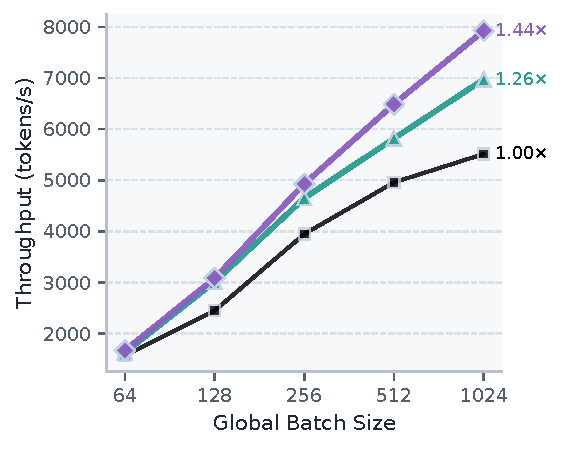
\includegraphics[width=0.31\textwidth]{main_res/30b_ep8_throughput.pdf}
    }
    \hfil
    \subfloat[{\parbox[c]{0.9\linewidth}{\centering Qwen3-30B-A3B (EP=32)}}]{
        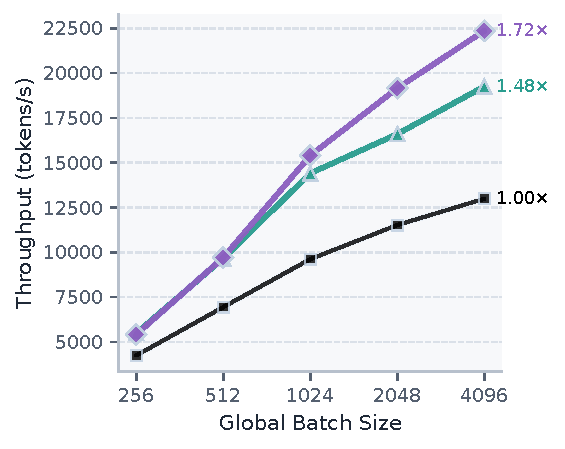
\includegraphics[width=0.31\textwidth]{main_res/30b_ep32_throughput.pdf}
    }
    \hfil
    \subfloat[{\parbox[c]{0.9\linewidth}{\centering Qwen3-235B-A22B (EP=32)}}]{
        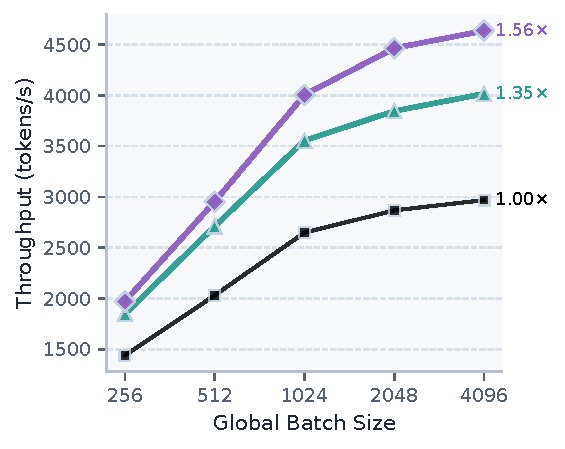
\includegraphics[width=0.31\textwidth]{main_res/235b_ep32_throughput.pdf}
    }

    \caption{
        End-to-end throughput on ShareGPT under different model scales and expert parallelism (EP) configurations.
        Spec-K consistently improves throughput over SpecDecode, achieving up to $1.72\times$ speedup.
        The gain becomes more pronounced at larger batch sizes and higher EP degrees, where communication and load imbalance dominate.
        The Lossless and Optimum policies are selected from the Pareto frontier of Qwen3-30B-A3B with Qwen3-0.6B, with average routing budgets $k=5.35$ and $k=4.91$, respectively.
    }
    \label{fig:throughput_end2end}
\end{figure*}

\subsection{Experimental Setup}

We evaluate Spec-K across a large design space spanning models, drafting methods, tasks, and system configurations. 
We therefore select representative settings that isolate key factors and reflect realistic serving scenarios.

\subsubsection{System Configuration}

Experiments are conducted on a multi-node GPU cluster with 8 NVIDIA H20 GPUs per node (96\,GB memory), connected via NVLink within each node and an NDR InfiniBand fabric across nodes. Each node is equipped with a 400\,Gb/s NVIDIA ConnectX-7 NIC.

All configurations use data parallelism (DP) for dense layers and expert parallelism (EP) for MoE layers, without tensor parallelism; only the expert-parallel degree varies.

Our implementation is based on vLLM~v0.16.0 with Triton-based GroupGEMM kernels and DeepEP~\cite{deepep2025} in low-latency mode (IBGDA). Prefix caching is disabled to ensure consistent performance and accuracy measurement. Speculative decoding uses padded drafter batches to minimize scheduling overhead. All methods, including the baseline, share the same system stack for fair comparison.

\subsubsection{Models and Drafting Methods}

We evaluate across multiple model families, including Qwen3~\cite{yang2025qwen3}, DeepSeek~\cite{liu2024deepseek}, and GLM~\cite{zeng2025glm}, covering scales from 30B to 671B parameters and both shared and non-shared expert architectures.

We consider three types of drafting methods: (1) small standalone language models, (2) EAGLE~\cite{li2024eagle} components, and (3) multi-token prediction (MTP~\cite{gloeckle2024better}). Unless otherwise specified, we use a speculation length of $\gamma = 3$, which is typical in practical deployments.

\subsubsection{Workloads and Tasks}

We evaluate both system performance and output quality using diverse generative workloads.

For system-level throughput, we use the ShareGPT dataset with vLLM's online serving benchmark, which reflects realistic conversational workloads.

For quality evaluation and policy calibration, we consider multiple task categories: (1) reasoning tasks (GSM8K-COT~\cite{cobbe2021gsm8k}, BBH-COT~\cite{suzgun2023bbh}), (2) code generation (HumanEval~\cite{chen2021humaneval}), and (3) instruction following (IFEval~\cite{zhou2023ifeval}). These tasks cover distinct generation regimes with different token-level characteristics, enabling a comprehensive assessment of adaptive allocation.

\subsubsection{Metrics}

We report end-to-end throughput (tokens per second) as the primary system metric. For speculative decoding, we measure the acceptance rate, defined as the ratio of accepted draft tokens to total proposed tokens.

We also evaluate weak scaling efficiency to assess distributed performance:
\[
\text{Efficiency} = \frac{\text{Throughput on } N}{\text{Throughput on } M \times (N/M)} \times 100\%.
\]

Unless otherwise specified, we fix all dimensions and vary a single factor (e.g., batch size or EP degree) to isolate system-level effects.

\begin{table}[!t]
\renewcommand{\arraystretch}{1.2}
\caption{Weak-scaling efficiency comparison.}
\label{table:scaling_performance}
\centering
\begin{tabular}{lcc}
\toprule
\textbf{Configuration} & \textbf{30B EP 8 $\rightarrow$ 32} & \textbf{235B EP 16 $\rightarrow$ 32} \\
 & (Local BS 64) & (Local BS 128) \\
\midrule
SpecDecode & 58.0\% & 88.5\% \\
Spec-K Lossless & 71.3\% & 92.5\% \\
Spec-K Optimum  & \textbf{73.8\%} & \textbf{94.0\%} \\
\bottomrule
\end{tabular}
\end{table}


\subsection{End-to-End System Performance} \label{sec:evaluation:end2end}

We evaluate end-to-end throughput using the ShareGPT dataset with vLLM's online serving benchmark. 
We control the global batch size via the maximum number of concurrent requests, and fix the maximum generation length to 1024 tokens to amortize prefill cost. 
We consider Qwen3-30B-A3B and Qwen3-235B-A22B as target models, paired with Qwen3-0.6B as the draft model, under different expert parallelism (EP) configurations. 
Throughput is measured as tokens per second over the entire serving process.

Figure~\ref{fig:throughput_end2end} shows that Spec-K consistently improves throughput across all batch sizes and system configurations. 
The Lossless and Optimum policies achieve up to $1.48\times$ and $1.72\times$ speedup over the SpecDecode baseline, respectively.
Notably, the improvement holds across both model scales and EP degrees, indicating that the benefit is robust to system and model variations.

The gain becomes more pronounced at larger batch sizes and higher EP degrees. 
In these regimes, system performance is increasingly dominated by communication overhead and load imbalance across experts. 
By reducing the per-token routing budget, Spec-K directly alleviates both effects, leading to larger relative speedups under high-throughput, highly distributed settings.

To further evaluate scalability, we measure weak scaling efficiency by fixing the per-device batch size while increasing the degree of expert parallelism. 
As shown in Table~\ref{table:scaling_performance}, Spec-K consistently achieves higher scaling efficiency than the baseline, with larger gains at higher parallelism levels. 
This suggests that Spec-K not only improves single-node efficiency, but also mitigates distributed inefficiencies that arise at scale.

\begin{figure}[!t]
    \centering

    
\includegraphics[width=0.6\linewidth]{latency_breakdown/legend.pdf}

    \vspace{-4mm}

    \subfloat[Qwen3-235B-A22B (EP=32)]{
        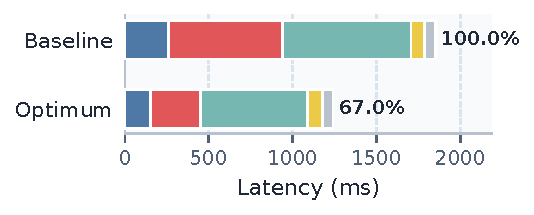
\includegraphics[width=0.8\linewidth]{latency_breakdown/235b_ep32.pdf}
        \label{fig:235b_ep32}
    }

    \vspace{-4mm}

    \subfloat[Qwen3-30B-A3B (EP=8)]{
        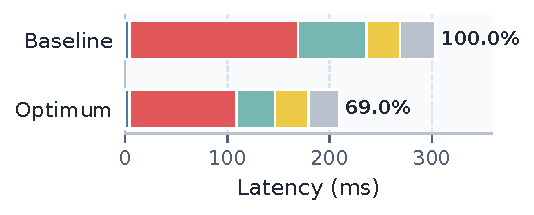
\includegraphics[width=0.8\linewidth]{latency_breakdown/30b_ep8.pdf}
        \label{fig:30b_ep8}
    }

    \caption{Latency breakdown of the verification step for SpecDecode and Spec-K (Optimum policy).
Spec-K reduces total latency in both settings, including computation (GroupGEMM) and aggregate communication (Dispatch and Combine).
The reduction closely follows the decrease in routing budget, with additional gains from improved kernel efficiency.}
    \label{fig:overall_latency_breakdown}
\end{figure}

\subsection{Where Does the Gain Come From?}

\subsubsection{Latency Breakdown}

To understand the source of the end-to-end speedup, we analyze the latency of the verification step, which dominates autoregressive decoding under speculative execution.

We profile the decoding of 32 tokens under offline inference with simultaneous request issuance to minimize scheduling effects. Two representative settings are considered: (1) Qwen3-30B-A3B with EP=8 at global batch size 1024 (intra-node), and (2) Qwen3-235B-A22B with EP=32 at global batch size 2048 (inter-node).

Figure~\ref{fig:overall_latency_breakdown} shows that Spec-K reduces total verification latency by 31\%--33\% in both settings. GroupGEMM and Combine latency decrease in both cases, and GroupGEMM speedup exceeds the theoretical expectation from average Top-$k$, indicating improved kernel efficiency under smaller expert sets.

Communication overhead is also reduced. In inter-node EP-32, Dispatch latency falls by 40.9\%, closely matching the 38.6\% reduction in routing volume; under intra-node NVLink, Dispatch is negligible. More importantly, Combine latency is $2.9\times$--$15.6\times$ that of Dispatch and falls by 16.4\%--43.7\% under Spec-K. Because Combine includes inter-device synchronization after expert computation, its substantial latency exposes the critical-path cost of EP load imbalance.

Table~\ref{tab:ep_load_balance} directly characterizes Spec-K's effect on EP load imbalance in an EP-32 GSM8K sweep. It reports two complementary metrics: busiest-device work, measured as the maximum number of token--expert assignments per target-model decode layer position and normalized to SpecDecode, and EP imbalance, measured as the maximum-to-mean assignment ratio across devices. Lossless and Optimum reduce busiest-device work to $0.68\times$ and $0.59\times$ of SpecDecode, respectively, while EP imbalance changes from $1.47\times$ to $1.55\times$. Thus, the busiest device receives substantially less work under both policies despite the modest increase in relative imbalance.

\begin{table}[!h]
\caption{EP-32 busiest-device work and load imbalance.}
\label{tab:ep_load_balance}
\centering
\small
\begin{tabular}{lccc}
\toprule
\textbf{Metric} & \textbf{Baseline} & \textbf{Lossless} & \textbf{Optimum} \\
\midrule
Busiest-device work & $1.00\times$ & $0.68\times$ & $0.59\times$ \\
EP imbalance (max/mean) & $1.47\times$ & $1.55\times$ & $1.55\times$ \\
\bottomrule
\end{tabular}
\end{table}

Overall, the components accelerated by Spec-K account for 80--90\% of the total verification latency, indicating that the method directly targets the dominant bottlenecks in the system. 
These results demonstrate that routing sparsity introduced by Spec-K translates effectively into both computation and communication savings at the system level.

\subsubsection{Effect on Acceptance Rate}

\begin{figure}[!t]
\centerline{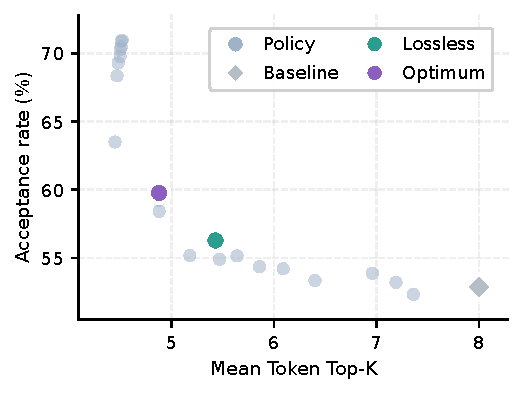
\includegraphics[width=0.8\linewidth]{total_topk_vs_acc.pdf}}
\caption{Acceptance rate versus average routing budget (Top-$k$) for Qwen3-30B-A3B with Qwen3-0.6B on ShareGPT.
Each point corresponds to a policy selected from the Pareto frontier.
Reducing the routing budget consistently increases acceptance across the evaluated Spec-K policies, revealing a coupled benefit of adaptive target-side routing.}
\label{fig:topk_vs_acceptance}
\end{figure}

\begin{figure*}[t]
    \centering

    
\includegraphics[width=0.475\textwidth]{pareto/legend.pdf}

    \vspace{-0.2cm}
    
    \subfloat[{\parbox[c]{0.9\linewidth}{\centering
Qwen3-30B-A3B, Qwen3-0.6B, GSM8K \\
Main configuration used throughout the paper
}}]{
        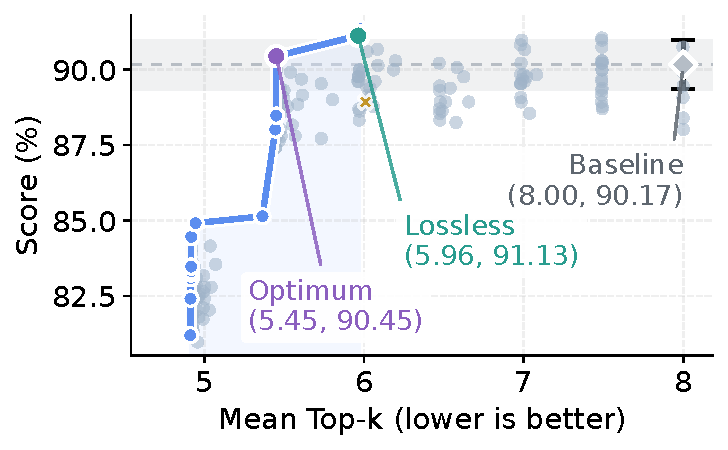
\includegraphics[width=0.31\textwidth]{pareto/30b_0b6_gsm8k_cot.pdf}
    }
    \hfil
    \subfloat[{\parbox[c]{0.9\linewidth}{\centering
Qwen3-30B-A3B-Instruct-2507, EAGLE, GSM8K \\
Non-reasoning model on a reasoning calibration
}}]{
        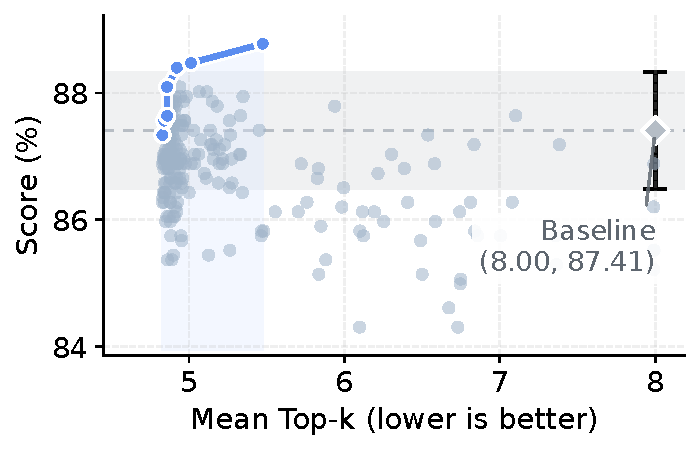
\includegraphics[width=0.31\textwidth]{pareto/30b_2507_eagle3_gsm8k_cot.pdf}
    }
    \hfil
    \subfloat[{\parbox[c]{0.9\linewidth}{\centering
Qwen3-30B-A3B-Instruct-2507, EAGLE, IFEval \\
Instruction following calibration
}}]{
        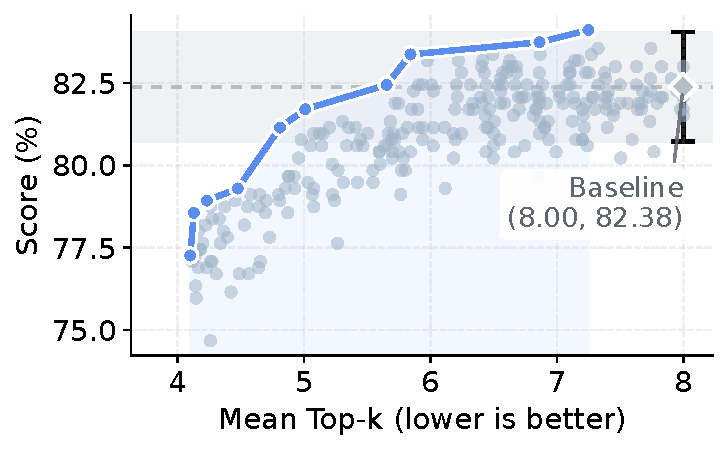
\includegraphics[width=0.31\textwidth]{pareto/30b_2507_eagle3_ifeval.pdf}
    }


    \subfloat[{\parbox[c]{0.9\linewidth}{\centering
Qwen3-30B-A3B, EAGLE, GSM8K \\
Ablation on drafting method
}}]{
        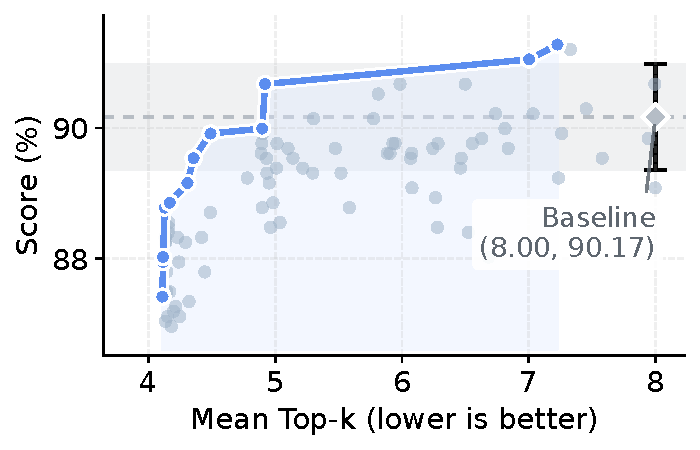
\includegraphics[width=0.31\textwidth]{pareto/30b_eagle3_gsm8k_cot.pdf}
    }
    \hfil
    \subfloat[{\parbox[c]{0.9\linewidth}{\centering
DeepSeek-R1, MTP, GSM8K \\
Large model with shared experts
}}]{
        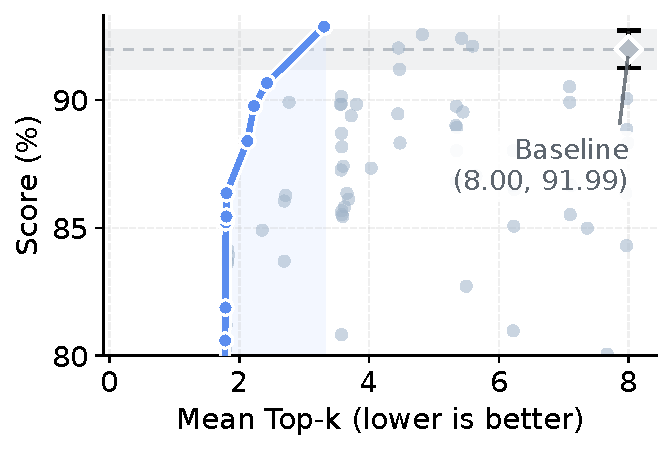
\includegraphics[width=0.31\textwidth]{pareto/r1_mtp_gsm8k_cot_8d_apply_last.pdf}
    }
    \hfil
    \subfloat[{\parbox[c]{0.9\linewidth}{\centering
GLM-4.7-Flash, MTP, GSM8K \\
Limited routing redundancy for $k=4$
}}]{
        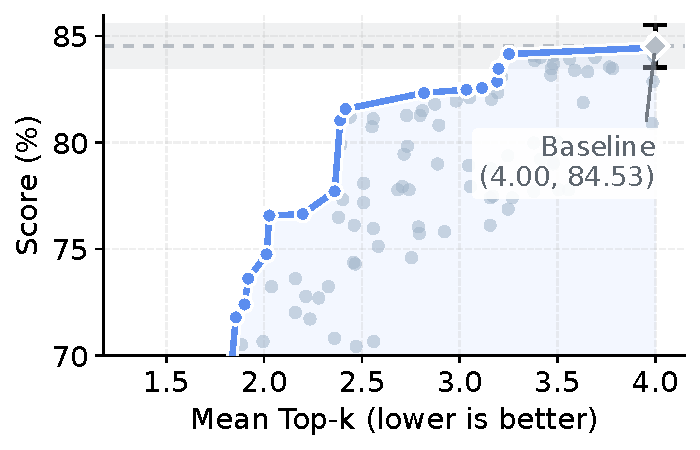
\includegraphics[width=0.31\textwidth]{pareto/glm47flash_mtp_gsm8k_cot.pdf}
    }

    \caption{Quality--efficiency Pareto frontiers across diverse model architectures, drafting methods, and tasks. The gray region and black error bar indicate the variability (±1 std) of the baseline; the three gold crosses in (a) mark fixed lower-layer controls.
All settings exhibit a consistent tradeoff structure: a plateau region with negligible quality loss followed by a sharp degradation beyond a critical routing threshold.
Spec-K identifies operating points along this frontier, including a lossless region and an optimal tradeoff point near the onset of the performance cliff.}
    \label{fig:frontiers}
\end{figure*}

In addition to reducing per-step latency, Spec-K also improves the efficiency of speculative decoding by increasing the acceptance rate.

To study this effect, we evaluate the relationship between the average routing budget and acceptance rate on Qwen3-30B-A3B with Qwen3-0.6B.
Each point corresponds to a policy selected from the Pareto frontier, executed on the ShareGPT dataset with a maximum generation length of 1024 tokens.

As shown in Figure~\ref{fig:topk_vs_acceptance}, reducing the average Top-$k$ leads to a consistent increase in acceptance rate.
This suggests that more aggressive routing improves alignment between the draft and target models, allowing more draft tokens to be accepted per step.

This trend is opposite to conventional expectations that reducing model capacity harms alignment, highlighting the unique effect of adaptive allocation.

This effect complements the reduction in per-step latency: reduced routing lowers the cost of each verification step, while higher acceptance increases the number of tokens committed per target-model step. The quality results in Section~\ref{sec:evaluation:pareto} further show that Spec-K can realize both gains with negligible target-model accuracy loss. Together, lower verification cost and higher acceptance contribute to the overall throughput improvement observed in Section~\ref{sec:evaluation:end2end}.

\subsection{Quality--Efficiency Tradeoff and Generalization}

\subsubsection{Comparison with Fixed-Layer Allocation}

To isolate the value of the preview signal, we construct fixed lower-layer policies that reduce the first $n$ MoE layers to a constant $k_{\mathrm{fixed}}$ and preserve the trained Top-$k$ in all later layers, without using draft perplexity. On Qwen3-30B-A3B with Qwen3-0.6B and GSM8K-COT, all three controls shown in Figure~\ref{fig:frontiers}(a) are dominated by the Spec-K frontier. At the high-quality end, a fixed policy scores 88.93 at average Top-$k$ 6.01, whereas Spec-K scores 91.36 at the lower Top-$k$ of 5.97. Unconditional layer reduction exposes some redundancy, but preview-guided allocation finds a better quality--efficiency tradeoff in the same model and evaluation stack.

\subsubsection{Cross-System Comparison with Lynx}

Lynx~\cite{gupta2024lynx} reports a $1.14\times$ speedup in median time per output token on Qwen3-30B-A3B-Instruct with GSM8K, with exact-match accuracy decreasing from 88.4\% to 87.6\%. Lynx remaps target-side routing decisions to reduce the active-expert set of a batch; Spec-K instead uses pre-execution draft signals to allocate token-wise routing budgets. The two methods therefore optimize complementary dimensions of MoE serving.

\subsubsection{Tradeoff Structure via Pareto Frontier} \label{sec:evaluation:pareto}

We analyze the quality--efficiency tradeoff of Spec-K across diverse model architectures, drafting methods, and tasks.

Figure~\ref{fig:frontiers} presents Pareto frontiers for six representative configurations spanning three model families (Qwen, DeepSeek, GLM), different drafting methods (standalone, EAGLE, and MTP), and both reasoning and instruction-following tasks.

Across all settings, we observe a consistent tradeoff structure: a plateau region where quality remains nearly unchanged as the Top-$k$ decreases, followed by a sharp degradation beyond a critical threshold. 
Spec-K identifies operating points along this frontier, including a \emph{lossless} region within the plateau and an \emph{optimal} point near the onset of the degradation cliff.

We further examine how this structure varies across different dimensions. 
First, comparing Figure~\ref{fig:frontiers}(a) and (d), we find that replacing the draft model with EAGLE yields a similar frontier shape and comparable optimal operating points, indicating that Spec-K is largely insensitive to the choice of drafting method.

Second, the frontier shape depends on the generation regime. 
For reasoning tasks such as GSM8K-COT, the plateau region is wide and exhibits a sharp transition, suggesting substantial redundancy in expert allocation. 
In contrast, for instruction-following tasks (IFEval), the frontier becomes smoother, with quality degrading gradually as the routing budget decreases. 
This reflects differences in token-level characteristics across decoding phases, where instruction-following requires stricter structural fidelity.

Finally, the degree of redundancy varies with model capacity and architecture. 
For example, DeepSeek-R1 exhibits a large lossless region, tolerating aggressive reductions in routing budget without quality degradation, whereas GLM-4.7-Flash shows a much narrower margin due to its smaller base Top-$k$. 
This indicates that the effectiveness of adaptive allocation depends on the inherent redundancy of the model.

Overall, these results show that while the exact tradeoff curve varies across settings, its structural pattern remains consistent, enabling Spec-K to reliably identify high-quality operating points across diverse scenarios.

\subsubsection{Cross-Task Transfer of Allocation Policies}

\begin{table}[t]
\centering
\setlength{\tabcolsep}{7pt}
\renewcommand{\arraystretch}{1.3}
\caption{Cross-task transfer of policies calibrated on GSM8K-COT (score / Top-$k$).}
\label{tab:transfer_accuracy}
\begin{tabular}{lccc}
\toprule
\textbf{Dataset} & \textbf{Baseline} & \textbf{Lossless} & \textbf{Optimum} \\
\midrule
GSM8K-COT {\scriptsize (Calibration)} & 90.17 / 8 & 89.86 / 5.72 & 89.09 / 5.16 \\

BBH-COT & 70.29 / 8 & 71.17 / 5.86 & 72.67 / 5.32 \\

IFEval {\scriptsize (Prompt Strict)} & 82.81 / 8 & 82.44 / 5.31 & 79.30 / 4.73 \\

HumanEval {\scriptsize (Pass@64)} & 54.88 / 8 & 60.37 / 5.51 & 67.68 / 4.86 \\

\bottomrule
\end{tabular}
\end{table}

We next evaluate whether a routing policy selected on a calibration task transfers to other downstream tasks.

We take the Lossless and Optimum policies identified on GSM8K-COT for Qwen3-30B-A3B with Qwen3-0.6B, and evaluate their accuracy across multiple benchmarks. 
Each result is averaged over five runs with different seeds to reduce evaluation variance.

As shown in Table~\ref{tab:transfer_accuracy}, the Lossless policy consistently preserves accuracy across all tasks, indicating that conservative allocation strategies generalize well. 
The Optimum policy achieves additional efficiency gains, while maintaining strong performance on reasoning (BBH-COT) and code generation (HumanEval) tasks.

However, on instruction-following tasks (IFEval), the Optimum policy exhibits a more noticeable degradation. 
This suggests that policies calibrated on reasoning tasks may be slightly over-aggressive when applied to tasks requiring strict structural adherence.

We attribute this behavior to differences in decoding phases. 
Reasoning tasks involve a ``thinking'' phase with higher uncertainty and redundancy, whereas instruction-following corresponds to a more constrained ``answering'' phase with lower tolerance for errors.
These differences imply that phase-aware allocation policies may further improve performance in practice. The vectorized execution path in Sec.~\ref{sec:implementation:policy-execution} allows separately calibrated policies to coexist within the same continuous batch.

Overall, these results show that routing policies learned from a single task transfer well across related workloads, while leaving room for further gains through phase-specific adaptation.

\subsection{Portability on Ascend NPUs}
\label{sec:evaluation:ascend}

We further evaluate Spec-K with vLLM-Ascend~\cite{huawei2024vllmascend} to study portability across accelerator and serving stacks. The experiment uses Qwen3-30B-A3B, a standalone Qwen3-0.6B draft model, and ShareGPT requests on an 8-NPU EP-8 deployment, with 7 draft candidates per verification step. Spec-K and SpecDecode use identical configurations at each offered load. Throughput is normalized to SpecDecode at 128 concurrent requests.

\begin{figure}[!h]
\centering
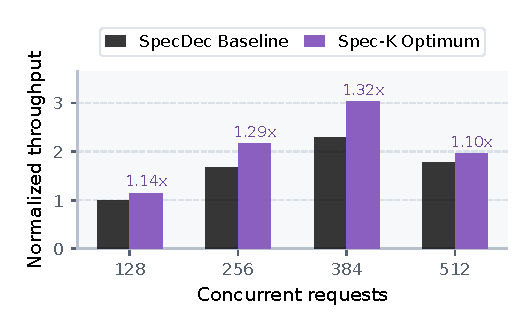
\includegraphics[width=\linewidth,trim=12bp 8bp 2bp 12bp,clip]{ascend/normalized_throughput.pdf}
\caption{Normalized end-to-end throughput on an 8-NPU Ascend platform, using SpecDecode at 128 concurrent requests as the common reference. Labels report Spec-K Optimum speedup; the 512-request setting experiences KV-cache capacity pressure.}
\label{fig:ascend_throughput}
\end{figure}

Figure~\ref{fig:ascend_throughput} shows end-to-end speedups of $1.14\times$, $1.29\times$, $1.32\times$, and $1.10\times$ across the four tested loads. The same preview-guided dynamic Top-$k$ mechanism therefore remains effective across a distinct accelerator and serving ecosystem, supporting the generality of Spec-K.


\section{Related Work}

\subsection{MoE Serving Systems}

Mixture-of-Experts (MoE) enables scalable LLMs via token-wise Top-$k$ routing, as established by GShard~\cite{lepikhin2020gshard} and Switch Transformer~\cite{fedus2022switch}. 
In serving, efficiency is dominated by expert parallelism overheads, including all-to-all communication, memory access, and load imbalance. 
Prior work addresses these bottlenecks through memory optimization~\cite{chen2025ktransformers,zhong2024adapmoe}, load balancing~\cite{deepseekai2025eplb,deepseek2025lplb}, communication--computation overlap~\cite{he2022fastermoe,liu2024deepseek}, and kernel design~\cite{gale2023megablocks}, with system frameworks integrating these techniques for large-scale deployment~\cite{rajbhandari2022deepspeed,li2023accelerating,hwang2023tutel,yuan2025x,kwon2023efficient,zheng2024sglang}.

These methods optimize execution under a fixed routing policy, typically assuming a uniform Top-$k$ budget across tokens. 
In contrast, we focus on token-level resource allocation and are orthogonal to system-level optimizations.

\subsection{Speculative Decoding}

Speculative decoding (SD) accelerates autoregressive generation by using a draft model to propose tokens that are verified in parallel by a target model. 
Prior work improves proposal quality and acceptance rates~\cite{stern2018blockwise,chen2023spec,leviathan2023spec,cai2024medusa,li2024eagle,miao2024specinfer,he2024rest,spector2023accelerating}, as well as batching and system efficiency.

Existing SD methods assume a fixed target-side computation pattern during verification. 
We instead use the draft model as a \emph{preview signal} to guide adaptive resource allocation before target execution, making our approach complementary to SD.

\subsection{Adaptive Computation and Dynamic Inference}

Adaptive inference dynamically adjusts computation based on input difficulty. 
Prior work spans both training-based and training-free approaches.

Training-based methods incorporate adaptivity into the model, including early exiting (e.g., BranchyNet~\cite{teerapittayanon2016branchynet}, DeeBERT~\cite{xin2020deebert}), token pruning~\cite{rao2021dynamicvit}, sparse attention~\cite{yuan2025native}, and learned MoE routing behaviors~\cite{zhou2022mixture,huang2024harder,jin2024moe++}. 
In particular, Harder Task Needs More Experts~\cite{huang2024harder} trains a confidence-based router with a dynamic sparsity objective.
These approaches rely on intrinsic signals such as intermediate activations and require retraining or architectural changes; Spec-K instead adapts a pretrained MoE model using a pre-execution draft signal.

Training-free methods adapt computation at inference time. 
Token pruning and KV-cache reduction (e.g., SnapKV~\cite{li2024snapkv}) reduce attention cost, while Lynx~\cite{gupta2024lynx} uses target-side router scores to remap low-affinity token--expert assignments onto a smaller batch-level active-expert set while preserving the model's per-token Top-$k$.
These approaches typically rely on signals observed during execution and operate at token, block, or batch granularity.

In contrast, Spec-K uses a draft signal available before target execution to vary each token's routing budget, reducing token--expert assignments themselves rather than only their batch-level union.

\section{Discussion and Conclusion}

Spec-K is an instantiation of a broader principle: \emph{resource allocation should be decided before execution, guided by predictive signals}. Formalized as RASP, this decouples \emph{difficulty estimation} from \emph{computation allocation}, enabling anticipatory adaptation using preview signals available prior to the target forward pass, without modifying model internals or incurring substantial runtime overhead.

Our results point to a consistent phenomenon: reducing the routing budget can improve both efficiency and speculative acceptance. This suggests that MoE inference operates in a regime of \emph{excess capacity but imperfect utilization}, where activating more experts does not necessarily improve draft--target alignment. Instead, adaptive sparsification acts as an implicit regularizer, suppressing low-contribution experts and yielding more consistent predictions. The observed Pareto structure---a wide plateau followed by a sharp degradation---indicates substantial redundancy for typical tokens, while a small subset of difficult tokens defines the capacity boundary. Spec-K exploits this asymmetry by reallocating resources toward high-uncertainty regions.

This approach has several limitations. Its effectiveness depends on preview signal quality; mismatch between draft uncertainty and true difficulty can lead to suboptimal allocation. Different generation regimes also exhibit varying sensitivity: policies calibrated on reasoning tasks may be over-aggressive for instruction-following workloads. Finally, our current calibration uses a uniform policy across layers, leaving finer-grained optimization unexplored.

These limitations suggest several directions. Richer preview signals (e.g., longer speculative windows) may better capture token difficulty. Extending allocation beyond token-level Top-$k$ to per-layer routing, attention sparsity, or other compute budgets would generalize RASP into a unified resource allocator. Further gains may also arise from co-design with scheduling, batching, and expert placement in distributed systems.

More broadly, RASP suggests a shift in how inference efficiency is approached. Instead of treating computation as a fixed per-token budget to be optimized post hoc, it becomes a quantity that can be \emph{predicted and allocated on demand}. In this view, Spec-K represents one point in a larger design space of online, signal-driven inference methods, where efficiency emerges not from uniformly reducing computation, but from aligning it with the structure of the generation process itself.

\section*{Acknowledgment}
We thank all anonymous reviewers for their constructive feedback. This work is supported by the National Natural Science Foundation of China under Grant No.~62372055, the National Science and Technology Major Project (2023ZD0120502), the School-Enterprise Cooperation Project of Beijing University of Posts and Telecommunications under Grant No.~A2025100, and the Fundamental Research Funds for the Central Universities. We also thank Huawei for providing Ascend NPU computing resources to support our generality and portability evaluations, and Fei Yi, Jie Meng, and Li Cao from Huawei for their insightful feedback.

\emph{For Antigone, for all the words that left unsaid.}


\bibliographystyle{IEEEtran}
\IEEEtriggeratref{50}
\bibliography{references}

\end{document}
